\documentclass{article}
\usepackage{multirow}
\usepackage{longtable}
\usepackage{float}
\usepackage{parskip}
\usepackage[margin=0.75in]{geometry}
\usepackage{pgfplots}
\usepackage{graphicx}
\pgfplotsset{compat=1.18}
\title{Assignment 1}
\author{Garvit Shah [U21CS089]}
\date{January 2023}
\begin{document}
   \maketitle

   \section*{Hardware Details}
   \begin{itemize}
    \item Memory: 8 GB 1600 MHz DDR3
    \item Processor: 1.8 GHz Dual-Core Intel Core i5
  \end{itemize}

  \section*{Software Details}
  \begin{itemize}
   \item Apple clang version 14.0.0 clang-1400.0.29.202
   \item xcode-select version 2395.
  \end{itemize}

   \section{Linear Search}
   \subsection{Algorithm}
   \begin{enumerate}
    \item Create a file pointer and Open the File
    \item Read the number from the file.
    \item Compare the number with the value to find.
    \item If found exit else continue reading the file.
   \end{enumerate}
   
   \subsection{Observations}
   \begin{table}[h!] 
   \centering     
   \begin{tabular}{ | p{3cm} | p{3cm} | p{3cm} | p{3cm} |  }  
    \hline
    \multicolumn{4}{|c|}{Time Complexity for Linear Search} \\
    \hline
    File Name & No. of Entries & Best Case & Worst Case\\
    \hline
    File-1 & 1,024 & 0.000003 & 0.000156\\
    File 2 & 4,096 & 0.000003 & 0.000644\\
    File 3 & 16,384 & 0.000003 & 0.002465\\
    File 4 & 65,536 & 0.000003 & 0.009768\\
    File 5 & 2,62,144 & 0.000003 & 0.037983\\
    File 6 & 10,48,576 & 0.000003 & 0.150615\\
    File 7 & 20,97,152 & 0.000003 & 0.302565\\
    File 8 & 41,94,304 & 0.000003 & 0.601808\\
    File 9 & 88,83,608 & 0.000003 & 1.202313\\
    File 10 & 167,77,216 & 0.000003 & 0.040706\\[1ex]
    \hline
   \end{tabular}
   \caption{Time taken for linear search}
\end{table}
\newpage
\subsection{Graph}
\begin{center}
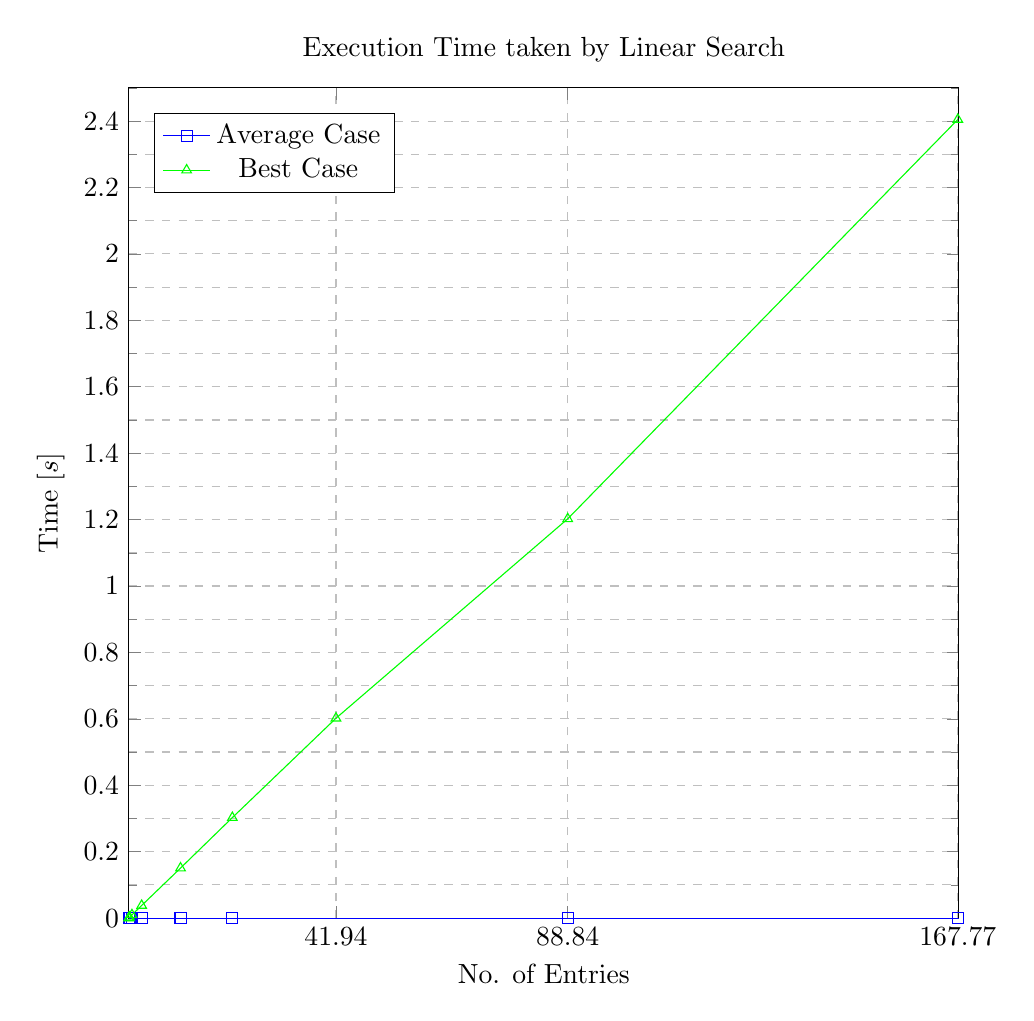
\begin{tikzpicture}
   \begin{axis}[
       title={Execution Time taken by Linear Search},
       xlabel={No. of Entries},
       ylabel={Time [\(s\)]},
       xmin=0, xmax=168,
       ymin=0, ymax=2.5,
       minor tick num = 1,
       height = \textwidth,
       width = \textwidth,
       xtick={41.94304,88.83608,167.77216},
       ytick={},
       legend pos=north west,
       grid=both,
       grid style=dashed,
   ]

   \addplot[
       color=blue,
       mark=square,
       ]
       coordinates {
       (0.01024,0.000003)(0.04096,0.000003)(0.16384,0.000003)(0.65536,0.000003)(2.62144,0.000003)(10.48576,0.000003)(20.97152,0.000003)(4194.304,0.000003)(88.83608,0.000003)(167.77216,0.000003)
       };      
   \addplot[
       color=green,
       mark=triangle,
       ]
       coordinates {
       (0.01024,0.000156)(0.04096,0.000644)(0.16384,0.002465)(0.65536,0.009768)(2.62144,0.037983)(10.48576,0.150615)(20.97152,0.302565)(41.94304,0.601808)(88.83608,1.202313)(167.77216,2.404731)
       };
    \legend{Average Case, Best Case}
   \end{axis}
   \end{tikzpicture}
\end{center}

\subsection{Conclusion}
The graph for the worst case is a straight line with some slope. A straight line implies that
the change in time taken is linearly dependent on the change in the no. of elements in the file,
as the line is given by $y = mx + c$.
Therefore, it can be concluded that the time complexity for linear search is $O(n)$.
Theoretically also time complexity comes out to be $O(n)$. Thus the conclusion matches to the theoretical
value of the time complexity.

\textbf{Time Complexity = $\theta(n)$}

\newpage
\section{Bubble Sort}
\subsection{Algorithm -}
\begin{enumerate}
 \item Create a file pointer and Open the File
 \item Insert the values into an array.
 \item Start two loops. Outer loop as number of elements in the array, inner as no. of elements - iterator
 \item Swap the elements if the current is bigger than the next.
\end{enumerate}
\subsection{Observations}
\begin{table}[h!] 
\centering     
\begin{tabular}{ | p{3cm} | p{3cm} | p{3cm} | p{3cm} | }  
 \hline
 \multicolumn{4}{|c|}{Time Complexity for Bubble Sort} \\
 \hline
 File Name & No. of Entries & Best Case & Average Case\\
 \hline
 File-1 & 1024 & 0.00348914 & 0.003746 \\ 
 File-2 & 4096 & 0.015065 & 0.056242 \\ 
 File-3 & 16384 & 0.238351 & 0.902742 \\ 
 File-4 & 65536 & 3.822212 & 14.473051 \\ 
 File-5 & 262144 & 80.9 & 231.703174 \\ 
 File-6 & 1048576 & 2635.25 & 3707.805908 \\ 
 File-7 & 2097152 & 7541 & 14831.596457 \\ 
 File-8 & 4194304 & 28163.8 & 59327.132655 \\ 
 File-9 & 8883608 & 120922 & 266143.099830 \\ 
 File-10 & 16777216 & 430619 & 949243.092676 \\[1ex]
 \hline
\end{tabular}
\caption{Time taken for bubble sort}
\end{table}
\newpage
\subsection{Graph}
\begin{center}
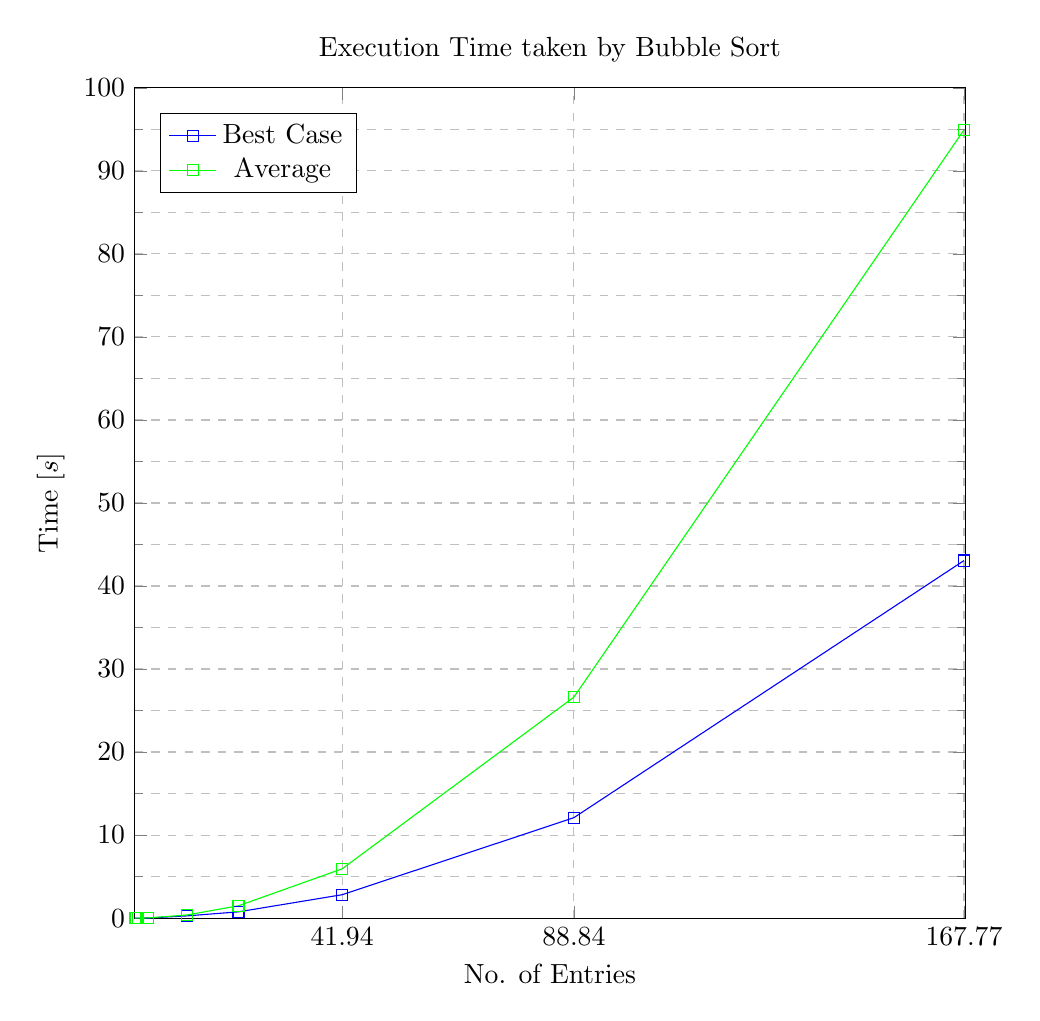
\begin{tikzpicture}
\begin{axis}[
    title={Execution Time taken by Bubble Sort},
    xlabel={No. of Entries},
    ylabel={Time [\(s\)]},
    xmin=0, xmax=168,
    ymin=0, ymax=100,
    xtick={41.94304,88.83608,167.77216},
    ytick={},
    minor tick num = 1,
    height = \textwidth,
    width = \textwidth,
    legend pos=north west,
    grid = both,
    grid style=dashed,
]
\addplot[
    color=blue,
    mark=square,
    ]
    coordinates {
    (0.01024,0.000000348914)(0.04096,0.0000015065)(0.16384,0.0000238351)(0.65536,0.0003822212)(2.62144,0.00809)(10.48576,0.263525)(20.97152,0.7541)(41.94304,2.81638)(88.83608,12.0922)(167.77216,43.0619)
    };

\addplot[
    color=green,
    mark=square,
    ]
    coordinates {
    (0.01024,0.0000003746)(0.04096,0.0000056242)(0.16384,0.0000902742)(0.65536,0.0014473051)(2.62144,0.0231703174)(10.48576,0.3707805908)(20.97152,1.4831596457)(41.94304,5.9327132655)(88.83608,26.6143099830)(167.77216,94.9243092676)
    };
    \legend{Best Case, Average}    
    
\end{axis}
\end{tikzpicture}
\end{center}
 
\subsection{Conclusion}
The graph for the worst case is a quadratic. A quadratic curve implies that
the change in time taken is quadratically dependent on the change in the no. of elements in the file,
as the line is given by $y = 4ax^2$.
Therefore, it can be concluded that the time complexity for Bubble Sort is $O(n^2)$.
Theoretically also time complexity comes out to be $O(n^2)$. Thus the conclusion matches to the theoretical
value of the time complexity.

\textbf{Time Complexity = $\theta(n^2)$}

\newpage
\section{Selection Sort}
\subsection{Algorithm -}
\begin{enumerate}
 \item Create a file pointer and Open the File
 \item Insert the values into an array.
 \item Start two loops. Outer loop as number of elements in the array, inner as no. of elements - iterator
 \item Find the minimum and place it at the index equal to the iterator.
\end{enumerate}
\subsection{Observations}
\begin{table}[h!] 
\centering     
\begin{tabular}{ | p{3cm} | p{3cm} | p{3cm} | p{3cm} |  }  
 \hline
 \multicolumn{4}{|c|}{Time Complexity for Selection Sort} \\
 \hline
 File Name & No. of Entries & Best Case & Average Case\\
 \hline
 File-1 & 1024 & 0.004686 & 0.004686 \\ 
File-2 & 4096 & 0.027157 & 0.047667 \\ 
File-3 & 16384 & 0.379485 & 0.785520 \\ 
File-4 & 65536 & 11.653376 & 12.791755 \\ 
File-5 & 262144 & 204.846 & 205.693883 \\ 
File-6 & 1048576 & 3200.145 & 3295.337373 \\ 
File-7 & 2097152 & 12800.532 & 13184.193533 \\ 
File-8 & 4194304 & 50732.0834 & 52742.471015 \\ 
File-9 & 8883608 & 303353.43523 & 236616.059310 \\ 
File-10 & 16777216 & 902341.14534 & 843947.960471 \\ [1ex]
 \hline
\end{tabular}
\caption{Time taken for selection sort}
\end{table}
\newpage
\subsection{Graph}
\begin{center}
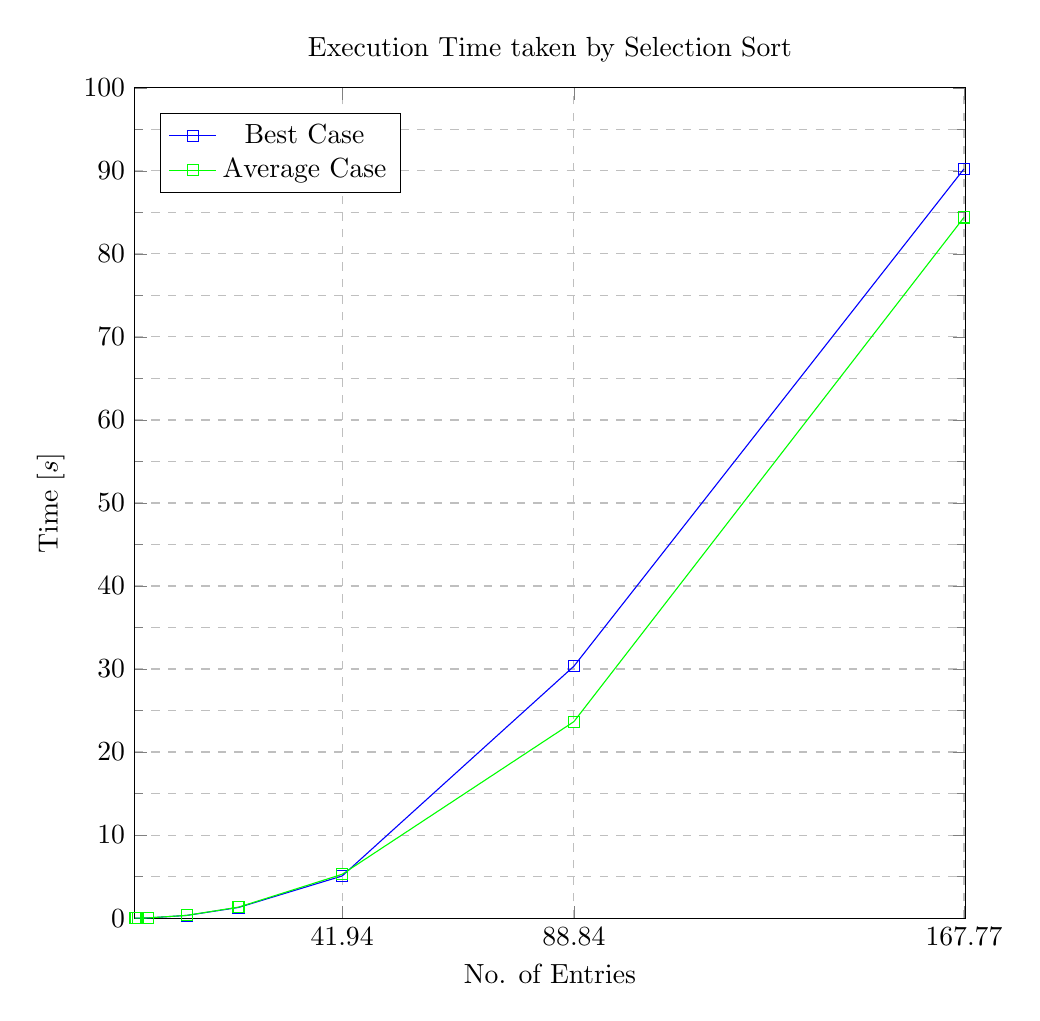
\begin{tikzpicture}
\begin{axis}[
    title={Execution Time taken by Selection Sort},
    xlabel={No. of Entries},
    ylabel={Time [\(s\)]},
    xmin=0, xmax=168,
    ymin=0, ymax=100,
    xtick={41.94304,88.83608,167.77216},
    ytick={},
    minor tick num = 1,
    height = \textwidth,
    width = \textwidth,
    legend pos=north west,
    grid=both,
    grid style=dashed,
]
\addplot[
    color=blue,
    mark=square,
    ]
    coordinates {
    (0.01024,0.0000004686)(0.04096,0.0000027157)(0.16384,0.0000379485)(0.65536,0.0011653376)(2.62144,0.0204846)(10.48576,0.3200145)(20.97152,1.2800532)(41.94304,5.07320834)(88.83608,30.335343523)(167.77216,90.234114534)
    };
\addplot[
    color=green,
    mark=square,
    ]
    coordinates {
    (0.01024,0.0000004686)(0.04096,0.0000047667)(0.16384,0.0000785520)(0.65536,0.0012791755)(2.62144,0.0205693883)(10.48576,0.3295337373)(20.97152,1.3184193533)(41.94304,5.2742471015)(88.83608,23.6616059310)(167.77216,84.3947960471)
    };
    \legend{Best Case, Average Case}    
    
\end{axis}
\end{tikzpicture}
\end{center}
 
\subsection{Conclusion}
The graph for the worst case is a quadratic. A quadratic curve implies that
the change in time taken is quadratically dependent on the change in the no. of elements in the file,
as the line is given by $y = 4ax^2$.
Therefore, it can be concluded that the time complexity for Selection Sort is $O(n^2)$.
Theoretically also time complexity comes out to be $O(n^2)$. Thus the conclusion matches to the theoretical
value of the time complexity.

\textbf{Time Complexity = $\theta(n^2)$}

\end{document}